\section{Characterization of operating environment}
\label{sect:character}

I have already stated (Sect.~\ref{sect:intro_background}) that the telescope operates in an \emph{uncertain environment}. In order to be able to make planning and scheduling decisions over the range of timescales outlined in Sect.~\ref{sect:pandstimescales} it will be neccessary to determine what constitute the components of this environment, to ascertain the range and variation of these components and to examine how such variation might impact on both the ability to schedule and the potential reward available. 
 
Though many of these processes are naturally unpredictable, it would be very useful to be able to at least have some way to determine the likeliness of these conditions occurring. If we could determine that the telescope would not be able to observe tomorrow, then we could ensure that an important observation was made tonight even though the potential reward might be better tomorrow. Conversely if we knew for certain that the telescope would be available tomorrow then we might make a low priority but urgent observation tonight and do the less urgent but higher priority observation tomorrow.

\subsection{Environment Components}
\label{sect:env_components}
The operating environment characteristics can usefully be broken down into the following components. Each of these can affect the operations of planning and scheduling in particular ways.

\begin{itemize}

\item {\bf Technical faults}. Mechanical, electrical, software and communications systems faults can leave the telescope unable to operate or may severely impair operational effectiveness. In some cases the telescope may be deliberately shutdown to permit preventative maintainance.

\item {\bf Bad weather}. Rain, high humidity, strong or gusting wind and calima (Saharan dust) can force the shutdown of the telescope systems to prevent damage to delicate instrument, optical and electrical hardware. The presence of ice prevents the dome from opening due to likely damage to the rams. Under any of these conditions, no observing is feasible. 

%  \begin{itemize}
%    \item rain can lead to ingress of water into delicate instrument, optical and electrical hardware.
%    \item high humidity may cause condensation on optical and electrical hardware.
%    \item high or gusting winds may damage the mechanical structure and tracking performance may be effected by wind-shake.
%    \item calima (Saharan dust) is a problem during the summer months causes damage to optical and mechanical systems.
%  \end{itemize}

\item {\bf Poor Sky conditions}. Do not pose problems for infrastructure but can severely disrupt the ability to perform useful observations. Extremly bad seeing, high extinction or high background sky-brightness lead to the requirement for longer exposures to achieve required signal-to-noise ratios (SNR\glossary{name={SNR},description={Signal to Noise ratio}}). In addition the pool of feasible observations is reduced as the conditions worsen leading to lower contention (easier scheduling task) but at the same time to reduced potential rewards.

\item {\bf Phase 2 population}. The actual content of the Phase 2 ODB affects how scheduling decisions are made. The distribution of the large number of its characteristics determines both the contention at any time and the potential rewards available. External software agents and users can modify the content of the Phase2 ODB at any time. Where these modifications occur during the night it seems reasonable to assume they will have some effect on the character and potential profitability of schedules which might be generated and introduce extra complexity into the scheduling operation.

\end{itemize}
  
\subsection{Technical faults}
The telescope is a complex system made up from numerous components. Though it has many inbuilt recovery mechanisms there are times when the overall system is unable to function without direct human intervention. Problems may occur with any of the following systems.

\begin{description}
\item [Mechanical] Physical problems with components such as:- main axes, focus drive, enclosure hydraulics, science fold deployment and instrument components such as filter-wheels and slides.

\item [Electrical] Power supplies to the site are occasionally disrupted though sometimes this information is available in advance.

\item [Network] Problems due to internal (inter-system) communications breakdown. These may be as simple as a wire dropping out, a software configuration problem or due to heavy network loading - typically a symptom of some other underlying problem. 

\item [Software] Low and high level systems can cause problems. These are highly complex systems and thus difficult to test thoroughly even with use of a simulated environment so problems can occur, particularly during upgrades. 

\end{description}

Several (7) years of knowledge gained from operating the telescope allow these errors to be classified into a few basic categories with differing timescales from inception to solution.

\begin{description}
\item [major catastrophe] These are problems which suddenly manifest themselves one night causing major downtime. Often these are due to mechanical breakdown of a component which requires a site visit to repair. The time involved can potentially be days if spares are not immediately available and no workround can be arranged. Where serious software failures occur, these are generally fixed within a day by a concentrated effort.

\item [occasional glitch] These are problems due to either non-terminal failure of a mechanical component which is too expensive to justify replacing or more often a known but difficult to repair software problem. The frequency of occurance and degree of impairment will tend to determine how much effort is employed on the solution.

\item [sporadic bug] Sometimes the problem is very difficult to identify and needs to occur many times before enough information is gathered to identify the cause. 

\item [shakedown] Effectively time required for new mechanical components or software deployments to bed in. Software in particular may be tested on the simulator but behave differently on the actual system due to subtle timing effects or unpredicted coincident situations.
\end{description}


\subsubsection{Source of data}
The main source for this information is the nightly logs kept by telescope operations staff\footnote{Obtainable from: http://telescope.livjm.ac.uk/News/Reports/}. These consist of the number of hours of technical downtime, weather downtime and actual observing per night. This information is assessed by a combination of examining system logs and from personal knowledge of the events of the previous night and so a degree of interpretation is involved. Of particular importance is the policy to assign the category \emph{weather downtime} to those periods when there was a combination of bad weather and technical problems - it is thus not possible to seperate these out. E.g. on a night where there might be 2 hours of observing mixed with 2 hours of intermittent technical problems followed by 6 hours of bad weather there is no way of telling whether the actual technical problem would have resulted in an additional period of downtime if the weather had remained good. 

Operations staff may assess early in the night that some serious technical problem is likely to affect the performance of the telescope during the night - e.g. poor image quality or tracking and decide to shutdown the telescope for the remainder of the night thus yielding an apparently high loss fraction rather than allow the automated systems to cycle between \emph{operational} and \emph{impaired} states.

Data covering a period of 30 months (919 days) for 2005, 2006 and part of 2007 was available and used to determine figures for probability of technical downtime and how this varies over the year. 

\subsubsection{Analysis}

Plots of technical downtime per night are displayed in Figs.~\ref{fig:nightly_tech2005}, \ref{fig:nightly_tech2006} and \ref{fig:nightly_tech2007}. The individual spikes represent the actual number of hours downtime on each specific night while the curved envelope reflects the variable night length over the course of the year. There does not appear to be any discernable pattern though as there is no sub-categorization of actual types of fault one cannot rule out the possibility that certain faults are more common in summer and others in winter, averaging out to a similar overall result. Basically, technical faults of some type can occur at any time.

\begin{figure}[htbp] 
\begin{center} 
 \subfigure[Technical downtime per night 2005.] {
    \includegraphics[scale=0.3, angle=-90]{figures/ecs/met_nightly_stats_tech2005.eps}   
    \label{fig:nightly_tech2005}
  }
 \subfigure[Technical downtime per night 2006.] {
    \includegraphics[scale=0.3, angle=-90]{figures/ecs/met_nightly_stats_tech2006.eps}  
    \label{fig:nightly_tech2006}
  } 
 \subfigure[Technical downtime per night 2007 (part).] {
    \includegraphics[scale=0.3, angle=-90]{figures/ecs/met_nightly_stats_tech2007.eps} 
    \label{fig:nightly_tech2007}
  }
\caption[Nightly variation of technical downtime for years 2005, 2006, 2007(part).]{Nightly variation (hours) of technical downtime for years 2005, 2006, 2007(part). Large blocks are empty due to operations policy preference for reporting bad weather downtime rather than technical when both occur simulataneously. The large empty block around February to March 2005 is due to a prolonged period of bad weather where no observing was possible.}
\end{center}
\label{fig:met_nightly_tech}
\end{figure}


Fig.~\ref{fig:tech_loss_dist} shows the distribution of fraction of night lost to technical problems, as can bee seen this is bimodal with around 72\% of nights suffering less than 5\% downtime (including those nights with zero loss). A total of 8\% of affected nights over the entire period suffered nearly 100\% downtime.  The variation of total technical downtime hours averaged by month for the available data is shown in Fig.~\ref{fig:monthly_tech_stats}. The average monthly downtime is 36.6 hrs over the period corresponding to about 1.2 hours per night.

\begin{figure}[htbp]  
  \begin{center}
    \includegraphics[scale=0.4, angle=-90]{figures/ecs/tech_loss_frac.eps}
  \end{center}
  \caption[Distribution of fraction of night lost to technical problems.]
   {Distribution of fraction of night lost to technical problems. Majority of nights (73\%) have less than 5\% loss, while some 8\% suffer near 100\% downtime.}
  \label{fig:tech_loss_dist}
\end{figure}

\begin{figure}[htbp]
  \begin{center}
    \includegraphics[scale=0.4, angle=-90]{figures/ecs/monthly_tech_stats.eps}
  \end{center}   
  \caption[Monthly averaged technical downtime.]
{Monthly averaged technical downtime (hours) over the period 2005 - 2007 (30 months). The data only includes periods where there was no weather downtime. Average time per month lost was 36.6 hrs or 1.2 hours per night}
  \label{fig:monthly_tech_stats}
\end{figure}


\subsubsection{Conclusions}
It had been hoped to look at lengths of runs of technical downtime to determine if there were any patterns - e.g. whether these occur in runs and with what distribution and frequency. Contamination of the data from weather downtime stats and the relatively small amount of data available makes this problematic. Heuristically however we might expect this to be the case. A problem might arise sporadically one night causing a degree of lost time, then maybe occurs the following night, spawning attempts by support staff to solve by software or engineering means. This may occur quickly or take several nights to correct, thereafter the problem disappears or becomes less frequent.

The diverse nature of these problems suggests that there is little chance of predicting future occurances - by their very nature they are unpredictable. The best that can realistically be achieved is to use the long term probabilities to estimate the likelihood of technical downtime over extended periods. 

Disruption to power supplies are sometimes known in advance and could be factored into medium term planning. Periods of planned maintainance are often known well in advance and could also be factored in. Prior to distribution of the Phase 2 entry system to users, both of these were implicitly taken account of by the operations team when setting up the content of the Phase 2 ODB but this information was not known explicitly by the scheduler.

\subsection{Weather}  
Weather statistics have been obtained from 3 independant sources.
\begin{itemize}
\item Data from the LT's own weather monitoring system (WMS\glossary{name={WMS},description={Weather Monitoring System}}) has been collected by embedded software over a 20 month period. 

\item Archived meteorological station data from various facilities at the ORM are available (\cite{sorensen02cat}) going back to 2002.

\item Observer reports of weather downtime hours per night (collated next day) for reporting on the telescope website. This data is bundled in with the technical downtime statistics and overrides these when both occur on the same night.
\end{itemize}


\subsubsection{Telescope Weather Monitoring System}%(XXX some basic info about the thing like who built it and what sensors it has).
 The Weather Monitoring System (WMS) provides feeds of various meteorological data from a weather station on site located 20m from the telescope enclosure.  Data is provided to the RCS at a cadence of around 5 seconds. The RCS filters this data and uses a set of rules (Table. \ref{tab:rcs_weather_rules}) to decide if the weather should be classified as \emph{good} in which case (all things being otherwise okay) observing may proceed, or \emph{bad} in which case observing may not proceed or if already underway should be stopped and the telescope and enclosure made safe.

Automated weather shutdowns based on WMS data are triggered by any of the following sources:-
\begin{itemize}
\item High humidity can lead to condensation on cold surfaces (mirror, electricals) and is an indicator of cloud and potential precipitation.
\item Rain causes wetting of all equipment, this has to be avoided especially on sensitive optical, electrical and hydraulic systems.
\item Moisture fraction is indicated by a digital sensor and indicates that rain or condensation is occuring or has recently occurred but not yet cleared sufficiently.
\item Cold temperatures lead to ice which can cause the enclosure portals to stick and thus put considerable strain on the motors and electrical supply if an attempt was made to open these.
\item Wind gusts  can cause damage to telescope structure and attached instruments. Moderate wind can also lead to poor tracking performance due to \emph{wind shake}.
\end{itemize}

Table \ref{tab:rcs_weather_rules} summarizes the rules in force (January 2008) for weather clear and alert triggers. Currently all rules have a 30 minute clearing stability time but this is a configurable parameter.

\begin{table}[htbp]
\begin{center}
\begin{tabular}{lllll}
\toprule
\multicolumn{5}{c}{Weather variable triggering conditions} \\
\midrule
Variable    & Alert            & Primary          & Secondary         & Stability \\
            & threshold        & clear level      & clear level       & parameter\\

\midrule
Humidity    &  $> 80$\%        & $< 70$\%         & $< 75$\%          & 30 min\\
Moisture    &  $> 10$\%        & $< 9$\%          & $< 9.5$\%         & 30 min\\
Wind speed  &  $> 15ms^{-1}$   & $< 12ms^{-1}$    & $< 14ms^{-1}$     & 30 min\\
Temperature &  $< 0.0^{\circ}$ & $> 0.1^{\circ}$C & $> 0.05^{\circ}$C & 30 min\\
\bottomrule
\end{tabular}
\end{center}
\caption[Definitions of alert and clear threshold levels for triggering good/bad weather conditions.]
{Definitions of alert and clear threshold levels for triggering good/bad weather conditions. A variable crossing its alert level signals bad weather. In order to clear (signal good weather) the variable must pass the primary clear level and remain below the secondary level for at least the time specified by the stability parameter. All variables must be in the \emph{clear} state for overall \emph{Good} weather. Any variable in its \emph{alert} state indicates \emph{bad} weather.}
\label{tab:rcs_weather_rules}
\end{table}

The data collected consists of 1582518 samples taken at around 30 seconds cadence over a period of 20 months between 2005 and 2007. The inter-sample gap distribution indicates that there are relatively few gaps. The vast majority of the samples occur with gaps of 30 seconds or less. A small number 292 exceed 5 minutes, a further 14 excede 30 minutes and 58 excede 60 minutes. The largest gap of 4.2 days occurred as a result of a site power outage
%\begin{figure}[htbp]
%  \begin{center}
%    \includegraphics[scale=0.4, angle=-90]{figures/ecs/gap_dist.eps}
%  \end{center}
%  \caption[Distribution of intersample gaps.]
%{Distribution of intersample gaps. The vast majority of the 1582518 samples occur with gaps of 30 seconds. A small number 292 excede 5 minutes, a further 14 excede 30 minutes and 58 excede 60 minutes. The largest gap of 4.2 days occurred during xxx as a result of a site power outage.}
%  \label{fig:gap_dist}
%\end{figure}


\subsubsection{Analysis of results}
\label{ss:weather_anal}
The distribution of humidity is shown in Fig.~\ref{fig:met_humidity_dist}. The distribution peaks around 15\% and average of 40\%. A very sharp secondary peak occurs around 95-100\% humidity. With the variable trigger levels (Sect.~\ref{tab:rcs_weather_rules}) set to 70\% (\emph{clear}) and 80\% (\emph{alert}) these can both be seen to be well into the tail of the main distribution just before the spike. This suggests that few false alerts should occur.

\begin{figure}[htbp]
  \begin{center}
    \includegraphics[scale=0.4, angle=-90]{figures/ecs/hum.eps}
  \end{center}
  \caption[Distribution of humidity at telescope site.]
{Distribution of atmospheric humidity at the telescope site over all samples. The distribution shows a profile with main peak around 15\% and average of 40\%. A very sharp secondary peak occurs around 95-100\% humidity. With the variable trigger levels set to 70\% good and 80\% bad these are in the tail of the distribution just before the spike level.}
  \label{fig:met_humidity_dist}
\end{figure}

% Moisture fraction
The distribution of moisture fraction is shown in Fig.~\ref{fig:met_moisture_dist}. The distribution is strongly peaked with average 0.07\%. A total of 89\% of measurements are below the alert level.

\begin{figure}[htbp]
\begin{center}
     \includegraphics[scale=0.4, angle=-90]{figures/ecs/moist.eps}
\end{center}
\caption[Distribution of moisture fraction at telescope site.]
{Distribution of moisture fraction at telescope site. Some 89\% of nights were below the alert threshold.}
\label{fig:met_moisture_dist}
\end{figure}




% Wind speed
The wind speed distribution is shown in Fig.~\ref{fig:met_windspeed_dist}. The distibution is wide with average 5.37$ms^{-1}$. Only 2\% of samples are above the alert level.

\begin{figure}[htbp]
\begin{center}
    \includegraphics[scale=0.4, angle=-90]{figures/ecs/wind.eps}
\end{center} 
\caption[Distribution of wind speed at telescope site.]
{Distribution of wind speed at telescope site. Only 2\% of nights were above the alert threshold.}
\label{fig:met_windspeed_dist}
\end{figure}

% Temperature
Fig.~\ref{fig:met_temp_dist} shows the distribution of external temperature at the site. The average temperature at the site is 9.43$^{\circ}$C. Only 3.7\% of time is the temperature below the alert level.

\begin{figure}[htbp]
\begin{center}
    \includegraphics[scale=0.4, angle=-90]{figures/ecs/temp.eps}
\end{center}  
\caption[Distribution of temperature at telescope site.]
{Distribution of temperature at telescope site. Average temperature over the year is $9.43^{\circ}$C with only 3.7\% of nights below the alert (freezing) temperature.}
 \label{fig:met_temp_dist}
\end{figure}


From (Table~\ref{tab:comp_meteo_trigs}) which shows the relative fractions of time when each of the weather triggers is within the alert region, it is clear that humidity is the greatest contributor to bad weather. The next highest is moisture level but these are quite closely related. Consequently it is reasonable to use humidity alone for any prediction studies.
\begin{table}[htbp]
\begin{center}
\begin{tabular}{ll}
\toprule
\multicolumn{2}{c}{Fraction of weather variable above alert trigger level} \\
\midrule
Variable & Fraction above alert level\\
\midrule
Humidity    & 18\%  \\
Moisture    & 11\%  \\
Wind speed  & 2\%   \\
Temperature & 3.7\% \\
\bottomrule
\end{tabular}
\end{center}
\caption[Fraction of recorded weather variable statistics over \emph{alert} level.]{Fraction of recorded weather variable statistics over \emph{alert} level. Humidity is the largest contributor at 18\%.}
\label{tab:comp_meteo_trigs}
\end{table}

Some examples of humidity profiles are presented in Figs.~\ref{fig:humidity_profile_examples}. It can be seen that on these individual nights there can be several periods of good and bad weather making forward planning difficult. Software was written to analyse the recorded data and generate statistics of good and bad weather periods based on the rules in Table.~\ref{tab:rcs_weather_rules}.

The results of this analysis are presented in Fig.~\ref{fig:wms_hum_frac_time} and shows the relative fraction of \emph{good} weather over various sized time bins. Bearing in mind the small period of data available (in climatological sense) there appears to be a tendency for better weather in summer (May-July) with increasingly higher fraction of bad weather in winter in accord with general observations.

Further analysis was performed on the WMS data to yield the distribution of lengths of good and bad weather periods. Fig.~\ref{fig:good_bad_hum_dist} shows the variation (i.e. number of periods) of lengths  of consecutive periods of good and bad weather based on humidity threshold (80\% trigger) and clearing stability time of 30 minutes. We see that shorter periods are most common with the average length of \emph{good} periods being 31.5 hours and bad periods being 7.7 hours. Cumulative plots are shown in Fig.~\ref{fig:good_bad_cumhum_dist}. The overall fraction of time classified as \emph{good} resulted in 80.03\% of all time with \emph{bad} weather making up the remainder. A rapid drop off suggests that long periods of continuous good/bad weather are rare, however outliers make this awkward as a source for prediction.

\begin{figure}[htbp]
\begin{center}
  \subfigure[Humidity profile 2007-01-29.] {
    \includegraphics[scale=0.25, angle=-90]{figures/ecs/hum_1_2007_01_29.eps}   
    \label{fig:hum_profile_2007_01_29}
  }
  \subfigure[Humidity profile 2007-02-20.] {
    \includegraphics[scale=0.25, angle=-90]{figures/ecs/hum_1_2007_02_20.eps}  
    \label{fig:hum_profile_2007_02_20}
  }
 \subfigure[Humidity profile 2007-03-26.] {
    \includegraphics[scale=0.25, angle=-90]{figures/ecs/hum_1_2007_03_26.eps}  
    \label{fig:hum_profile_2007_03_26}
  }
 \subfigure[Humidity profile 2007-03-28.] {
    \includegraphics[scale=0.25, angle=-90]{figures/ecs/hum_1_2007_03_28.eps}  
    \label{fig:hum_profile_2007_03_28}
  }
 \subfigure[Humidity profile 2007-04-15.] {
    \includegraphics[scale=0.25, angle=-90]{figures/ecs/hum_1_2007_04_15.eps}  
    \label{fig:hum_profile_2007_04_15}
  }
 \subfigure[Humidity profile 2007-04-16.] {
    \includegraphics[scale=0.25, angle=-90]{figures/ecs/hum_1_2007_04_16.eps}  
    \label{fig:hum_profile_2007_04_16}
  }
\end{center}  
\caption[Examples of humidity profiles.]{Example humidity profiles. As can be seen there is some considerable variation from night to night. Humidity can suddenly rise from what looks like a stable low level through the alert level in avery short period of time. This is often due to cloud spilling over the rim of the caldera.}
\label{fig:humidity_profile_examples}
\end{figure}

\begin{figure}[htbp]
\begin{center}
    \includegraphics[scale=0.4, angle=-90]{figures/ecs/hum_frac_time.eps}
\end{center} 
\caption[Monthly averaged good weather fraction based on humidity level.]
{Monthly averaged good weather fraction ($1-\Delta_W$) over the period 2005-2007 (20 months) based on WMS humidity levels averaged with various bin sizes. There is considerable month to month variation but summer generally has the highest fraction of good weather.} 
\label{fig:wms_hum_frac_time}
\end{figure}



\begin{figure}[htbp] 
\begin{center}
    \includegraphics[scale=0.4, angle=-90]{figures/ecs/good_bad_hum_bin.eps}
\end{center}
\caption[Relative probability of lengths of good/bad weather runs.]
{Relative probability of lengths of good/bad weather runs. Though around half the continuous periods of good or bad weather are less than 1 hour, there is a considerable tail in the distribution.}
\label{fig:good_bad_hum_dist}
\end{figure}

\begin{figure}[htbp] 
\begin{center}
    \includegraphics[scale=0.4, angle=-90]{figures/ecs/good_bad_cumhum_bin.eps}
\end{center}
\caption[Cumulative probability of lengths of good/bad weather runs.]
{Cumulative probability of lengths of good/bad weather runs. Only 5\% of bad runs last more than 10 hours while some 20\% of good runs last 10 hours or more.}
\label{fig:good_bad_cumhum_dist}
\end{figure}

%Idea behind these is something like: If we are $x$ hours into a period of good humidity then based on the known distribution of lengths the end of that period is approaching and the probability of this occurring in the next $y$ hours is given by integrating the PDF appropriately from $t=x$ to $t=y$. This will on average give the correct probability but for subsequent days we may do just as well using climatological statistics.

\subsubsection{Prediction experiment}
\label{ss:conc_pred}
If we wish to factor weather statistics into the planning and scheduling decision making processes, then without additional information the best we can do is to use the long-term climatological prediction. Based on the data plotted in Fig. {\ref{fig:good_bad_period_time} showing the lengths of periods of continuous \emph{good} and \emph{bad} weather, a simple prediction model was tested based on the assumption that the weather will continue in its current state for a period roughly equal to the length of time it has already been in that state continuously, thereafter the probability of maintaining this state would decrease at an assumed exponential rate with a decay length some multiple of the current stability period. As an example, assume the weather has been \emph{good} for about $\tau$ hours. We then assume it will continue to remain \emph{good} for about another $\tau$ hours with the probability decaying as $e^{-t/m\tau}$, $m$ being a scale factor yet to be determined.

\begin{figure}[htbp]
\begin{center}
    \includegraphics[scale=0.4, angle=-90]{figures/ecs/gbc_period.eps}
\end{center}
\caption[Time variation of lengths of good/bad periods based on humidity level.]
{Time variation of lengths of good/bad periods based on humidity level. There are more longer periods of good weather than bad. This information was used to setup an experiment to test the ability to predict weather based on the length of time in a particular state using Eqn.~\ref{eqn:prediction_decay}.}
\label{fig:good_bad_period_time}
\end{figure}

A set of simulations were run using the extracted period data (Fig. {\ref{fig:good_bad_period_time}) to determine the effectiveness of this prediction mechanism. Every 15 minutes through the available period a determination is made of the current weather state and how long ($\tau_G$ \emph{good}\notation{name={$\tau_G$},description={Length of time conditions remain \emph{good}},sort={T}}) or ($\tau_B$ \emph{bad}\notation{name={$\tau_B$},description={Length of time conditions remain \emph{bad}},sort={T}}) it has been in that state. A prediction is made at a number steps into the future (192 steps of 15 minutes constituting up to 48 hours look-ahead) using the rule specified in Eq.~(\ref{eqn:prediction_decay}). At each step the prediction is compared to the actual weather state at the time and counted as either a hit (correct prediction) or miss (incorrect prediction). The final percentages shown in Fig. \ref{fig:gbc_prediction} against look-ahead time for a number of decay scale factors $m$. The baseline of 80.03\% represents the worst we should be able to acheive on average based on long-term climatological prediction - basically if we always just guess that the weather will be good this will work 80.03\% of the time. Fig. \ref{fig:gbc_m_crossover} shows the crossover point - the length of look-ahead where the prediction becomes worse than long-term climatological prediction as a function of the decay scale factor $m$. This is seen to converge towards a value of 30-31 hours which is close to the average length of \emph{good} weather period.

\begin{equation}
\label{eqn:prediction_decay}
P_{good}(\Delta T) = 
\begin{cases} 
\Delta T < \tau_G : & 1   \\ 
\Delta T > \tau_G, \tau_G < T_G : & e^{\frac{\Delta T-\tau_G}{m \tau_G}} \\
\Delta T > \tau_G , \tau_G > T_G : & e^{\frac{\Delta T-T_G}{m \tau_G-T_G}}
\end{cases}
\end{equation}



\begin{figure}[htbp] 
  \begin{center}
    \includegraphics[scale=0.4, angle=-90]{figures/ecs/gbc_predict.eps}
  \end{center}
  \caption[Accuracy of look-ahead weather prediction using time decay model]
  {Effect of time scaling-factor ($m$) on variation of prediction accuracy of time decay prediction model against look-ahead time. All plots show a decay with time. As the scale factor is increased the cross-over point for the prediction against climatological baseline prediction of 80.03\% approaches a maximum of around 31 hours. }
  \label{fig:gbc_prediction}
\end{figure}

\begin{figure}[htbp]
  \begin{center}
    \includegraphics[scale=0.4, angle=-90]{figures/ecs/m_crossover.eps}
  \end{center}   
  \caption[Variation of cross-over point for look-ahead weather prediction using time decay model with scale factor.]
  {Variation of cross-over point for look-ahead weather prediction using time decay model with scale factor.}
  \label{fig:gbc_m_crossover}
\end{figure}



% some graphs showing the data for 2005 2006 2007 

\subsubsection{Observer reports}
The observer-reported hours-per-night data for weather downtime are displayed in figures \ref{fig:nightly_weather2005} for 2005 , \ref{fig:nightly_weather2006} for 2006  and \ref{fig:nightly_weather2007} for 2007 (part).

Figure (\ref{fig:ecs_monthly_weather_stats}) shows the variation of weather downtime fraction, the fraction of the potential observing hours per night lost to bad weather ($\Delta_W$\notation{name={$\Delta_W$},description={Fraction of night during which weather conditions are {\bf not} acceptable for observing},sort={W}}) averaged by month for the available data. June is the best month with less than 10\% of potential observing time lost to weather. February is worst with 58\% of potential observing time lost to weather.

%The observing hours per night are displayed in figures \ref{fig:nightly_obs2005} for 2005, \ref{fig:nightly_obs2006} for 2006 and\ref{fig:nightly_obs2007} for 2007 (part).

\begin{figure}[htbp]
\begin{center}
    \includegraphics[scale=0.4, angle=-90]{figures/ecs/monthly_weather_stats.eps}
\end{center}   
\caption[Monthly averaged weather downtime fraction.]
{Monthly averaged weather downtime fraction over the period 2005 - 2007 (30 months).}
 \label{fig:ecs_monthly_weather_stats}
\end{figure}


%\clearpage
\begin{figure}[htbp]
\begin{center}
 \subfigure[Weather downtime per night 2005.] {
      \includegraphics[scale=0.3, angle=-90]{figures/ecs/met_nightly_stats_weather2005.eps}
      \label{fig:nightly_weather2005}
  }
 \subfigure[Weather downtime per night 2006.] {
      \includegraphics[scale=0.3, angle=-90]{figures/ecs/met_nightly_stats_weather2006.eps}
      \label{fig:nightly_weather2006}
  } 
 \subfigure[Weather downtime per night 2007.] {
     \includegraphics[scale=0.3, angle=-90]{figures/ecs/met_nightly_stats_weather2007.eps}
     \label{fig:nightly_weather2007}
  }
\end{center}
\caption[Bad weather periods for years 2005, 2006, 2007(part).]
{Nightly plots for bad weather periods (hours) for years 2005, 2006, 2007(part). There is clearly more good weather in the summer months.}  
\label{fig:met_nightly_weather}
\end{figure}


%\clearpage
%\begin{figure}[htbp]
%\begin{center}
% \subfigure[Observing hours per night 2005.] {
%     \includegraphics[scale=0.3, angle=-90]{figures/ecs/met_nightly_stats_obs2005.eps}   
%     \label{fig:nightly_obs2005}
%  }
% \subfigure[Observing hours per night 2006.] {
%     \includegraphics[scale=0.3, angle=-90]{figures/ecs/met_nightly_stats_obs2006.eps}     
%     \label{fig:nightly_obs2006}
%  } 
% \subfigure[Observing hours per night 2007.] {
%     \includegraphics[scale=0.3, angle=-90]{figures/ecs/met_nightly_stats_obs2007.eps} 
%     \label{fig:nightly_obs2007}
%  } 
%\end{center}
%\caption{Nightly hours plots for observing time for years 2005, 2006, 2007(part)}
%\label{fig:met_nightly_obs}
%\end{figure}



\subsubsection{Analysis}
This data is subject to human interpretation. There is no hour by hour detail, only nightly totals. There is also no combination data (when bad weather and technical downtime occur simultaneously). Additionally there is a bias such that when combinations do occur, this is logged as bad weather. The plots do reveal a tendency for better weather in summer and more bad weather in winter as might be expected but beyond that little of use in prediction. Plots of run lengths, consecutive days where the  fraction of time lost to bad weather exceed given thresholds, are shown in Figure~\ref{fig:ecs_run_len}. We see that shorter runs of good and bad weather are more common 

Using this plot one can predict the likely length of a current run of bad weather based on the length up to the present time using Bayes theorem E.g. if the current run is 2 days long so far, the probability of the run going on for another 12 days or more is P(14)/P(2) = 0.23.


\begin{figure}[htbp]
\begin{center}
    \includegraphics[scale=0.4, angle=-90]{figures/ecs/run_len_thresh.eps}
\end{center}
\caption[Cumulative probability of lengths of bad weather runs for variable threshold value.]
{Probability of the length of a run of continuous bad weather for bad weather fraction ($\Delta_W$) exceding threshold values between 0 and 1. Using this plot it is possible to determine the the likely length of the current bad weather run based on the length of run to-date.}
\label{fig:ecs_run_len}
\end{figure}



\subsubsection{Conclusions}
Meteorological information obtained from logs of the telescope's own weather monitoring system (WMS) and from nightly observing logs was analyses and it was found to be suitable for observing for about 80\% of the time averaged over the year. There is generally more good weather in summer than winter with $<5$\% bad weather in June rising to as much as 60\% in February. The major contribution to bad weather is high humidity accounting for around 90\% of such time. Other factors such as high winds and freezing temperatures account for only a few percent of the bad weather. 

Using an analysis of the distribution of lengths of good and bad periods, a simple prediction model was designed and tested against recorded data. It was found capable of anticipating the length of the current period of weather with a degree of accuracy exceeding the long-term average for up to 30 hours ahead though the accuracy decreased with look-ahead time. 

Further analysis shows that in runs of continuous bad weather around 50\% of bad weather runs are $<5$ days long with $<10$\% of runs exceeding 15 days. This information could be useful in longer-horizon planning.


%typically we need to answer questions like:
%\begin{itemize}
%\item What are the chances I can do G in 3 hours as I will get a better quality observation then compared to now - basic utility theory gives us the way to trade off uncertainty in future rewards against certainty at present. 
%\item What are the chances of performing X in the next 3 days - I can do X on any of those nights with little difference in reward but if I do X tonight I miss my chance of doing Y.
%\item What are the predicted effects on data yield over the next N nights on group Z based on likelihood of execution on those nights.
%\end{itemize}

\subsection{Atmospheric Seeing and Extinction}  
\label{sect:sub_atmoseeing}
The atmospheric seeing regime has been studied for many years both through short campaigns and as part of longer studies aimed at site testing for telescopes such as the Grande Telescopio Canarias (GTC\glossary{name={GTC}, description={Grand Telescopio Canarias - a telescope at the ORM}}).
 A short study in 1990 by \citet{vernin92optical} using equipment at the Nordic Optical Telescope site (NOT\glossary{name={NOT},description={Nordic Optical Telescope - a telescope at the ORM},sort={N}}) on the contributions of the various air layers above the site suggests that the main contribution, some 50\%, comes from air in the boundary layer (from a few meters to 1 km above the ground. They found that 40\% is provided by the free air above 1 km and that 8\% comes from the surface layer of the first few meters. Sources internal to the dome provide the remaining 2\%.

A longer 9 month study \citep{munoz97nighttime} using a DIMM mounted on a 5m tower (above the surface layer) concluded that the inversion layer which lies below the observatory site is of particular importance in determining seeing characteristics. The layer generally lies between 1200m and 1500m, well below the site at 2400m and acts to suppress convection - a layer of strato-cumulus is generally seen at the top of this layer. Around 55\% of the local atmospheric humidity is trapped below the layer with around 20\% above. They find that the best seeing correlates with those times when the inversion layer is at its lowest (around 1200m) and strongest (largest temperature difference between top and bottom of the layer) which occurs in the summer months (June, July and August). At this time the strength of the trade winds is highest. They find that during the summer the average seeing is 0.61'' and median 0.5''. During the remaining months the average seeing is 0.77'' and median 0.91''. 

\citet{munoz97nighttime} also studied some time variation effects finding that typically seeing can change very abruptly, deteriorating within a few minutes but that it rarely returns to a stable level so quickly. Typically they find a recovery time of around 2 hours which they put this down to the effects of sudden perturbations in a steady atmospheric flow giving rise to turbulence which can take some time to settle. Some oscillatory effects were recorded with a period of around 45 minutes. 

A year long study by \citet{munoz98homogeneity} on the variation of seeing between different sites at the ORM revealed an average seeing of 0.72'' and median 0.65''. They found relatively small variation between sites except when the seeing was particularly poor when the variation was more pronounced - up to 0.2'' between locations. In summer they find that seeing is better than 0.5'' for 50\% of the time dropping to 25\% averaged over the whole year. A correlation was found between wind speed and direction and seeing quality. 

At low wind speed ($<$ 5 km/h) there was no relation between wind direction and seeing. At medium wind speed (5 - 15 km/h) they found the best seeing associated with Northerly winds and poor seeing when the wind was Southerly (from over the Caldera rim). At high wind speeds ($>$ 45km) seeing was generally very poor. 

In a further study of site conditions, \citet{vernin98temporal} find a relaxation time for seeing to return to \emph{normal} after an excursion to be around 1.2 hours.

%More recently \citet{trinquet06model} have devised a model (AXP) to derive seeing estimates from meteorological data. They find the probability of estimating the seeing with $<30$\% error is around 58\% as compared to 41\% for the $C^2_N$ model citep{} and 36\% for the Vernin-Tatarski model \citep{vernin}

\subsubsection{Collected seeing data from archived images}
\label{sect:collseedata}

Data from the LT image archive, originally extracted from FITS \glossary{name={FITS},description={Flexible Image Transport System - an astronomical data file specification}}headers was collated and processed to give seeing statistics. The processing included correcting for target zenith distance $z$ and wavelength $\lambda$ (Eq.~\ref{eq:seeing_corr})\footnote{The correction of seeing to R-band ($\lambda_R$) at zenith is due to work by \citet {sarazin90eso} based on earlier work by \citet{fried66optical}} using details of the instrument filter choice, correction for binning and removal of outliers caused by:- \begin{inparaenum}[(\itshape i\upshape )]
\item Some images are deliberately defocussed or telescope out of focus,
\item Images of extended sources cause problems for reduction pipeline,
\item Other general pipeline problems.
\end{inparaenum} 

\begin{equation}
  s(z=0,\lambda_R) = s(z,\lambda) (\frac{\lambda}{\lambda_R})^{-0.2}\sec^{0.6}z
\label{eq:seeing_corr}
\end{equation}

The number of images available for processing per month are shown in Fig.~\ref{fig:monthly_seeing_count}. There are at least 2000 images per month, in some cases up to 11000. On average around 5000 giving a worst case statistical noise of around $\pm 2.2$\%. 

\begin{figure}[htbp]
\begin{center}
    \includegraphics[scale=0.4, angle=-90]{figures/ecs/corr_monthly_bins.eps}
\end{center} 
\caption[Monthly count of images used for deriving seeing statistics.]
{Monthly count of images used for deriving seeing statistics. There are at least 2000 samples available on each of the months with a maximum of 11000.}
\label{fig:monthly_seeing_count}
\end{figure}


Figures \ref{fig:see_dist} and \ref{fig:see_cum_dist} show the relative and cumulative distributions of atmospheric seeing over the full period of available images both raw and corrected for elevation and wavelength. Table \ref{tab:seeing_quartiles} shows the quartiles of seeing data. 

\begin{figure}[htbp]
\begin{center}
    \includegraphics[scale=0.4, angle=-90]{figures/ecs/seeing_dist.eps}
\end{center} 
\caption[Relative distribution of r-band seeing data.] {Relative distribution of r-band seeing data. For raw images the average seeing is 1.35''while for corrected images this reduces to 0.98''. Both distributions are broad with 50\% of raw images between 0.97'' and 1.63'' while for corrected images 50\% of images lie between 0.8'' and 1.3''.}
\label{fig:see_dist}
\end{figure}

\begin{figure}[htbp]
\begin{center}
    \includegraphics[scale=0.4, angle=-90]{figures/ecs/cum_seeing_dist.eps}
\end{center}  
\caption[Cumulative distribution of r-band seeing data.]
{Cumulative distribution of seeing data.}
\label{fig:see_cum_dist}
\end{figure}


\begin{table}[htbp]
\begin{center}
\begin{tabular}{lllll}
\toprule
\multicolumn{3}{c}{Seeing quartiles (r-band)} \\
\midrule
Quartile & Raw & Corrected \\
\midrule
Q1 & 0.97'' & 0.8''  \\
Q2 & 1.25'' & 0.95'' \\
Q3 & 1.63'' & 1.3''  \\
\bottomrule
\end{tabular}
\end{center}
\caption[Quartiles of raw and corrected seeing distributions]
{Quartiles of raw and corrected seeing distributions extracted from Fig.~\ref{fig:see_dist}}
\label{tab:seeing_quartiles}
\end{table}

%Following \cite{racine96temporal} a plot of FSC is displayed in Fig.~\ref{fig:fsc}

%\begin{figure}[htbp]
%\begin{center}
%    \includegraphics[scale=0.4, angle=-90]{figures/ecs/fsc.eps}
%\end{center} 
%\caption[Fractional seeing change (FSC) after \cite{racine96temporal}.]
%{Fractional seeing change (FSC) after \cite{racine96temporal}. This is an indication of the change in seeing between pairs of images taken at varying intervals averaged over all available images.}
%\label{fig:fsc}
%\end{figure}

\subsubsection{Variation of seeing during the night.}
It is a common belief that there is a systematic variation in seeing quality during the night, This has been found to be incorrect by \citet{munoz97nighttime}. The data collected and displayed in Fig.\ref{fig:ut_av_seeing} shows the variation of average seeing with time (binned by UT) over a 3 year period. Allowing for the variation of a given UT time with \emph{time after sunset} over the year there does not appear to be a large variation over the darker part of the night. Fig.~\ref{fig:ut_bin_count} shows the relative number of samples per UT bin, typically around 1500 samples per bin indicating low levels of noise (around $\pm 2.5$\%). Fig.~\ref{fig:see_profile_examples} shows some examples of nightly seeing profiles. On any individual night the seeing may increase, decrease, remain relatively stable or vary quite dramatically.

%XXX [Add some example nightly seeing plots here same format 6 on a page as humidity samples]



\begin{figure}[htbp]
\begin{center}
    \includegraphics[scale=0.4, angle=-90]{figures/ecs/corr_see_ut.eps}
\end{center} 
\caption[R-band seeing averaged by UT binning of time over all available nights.]
{Seeing averaged by UT binning of time over all available nights. There is clearly no systematic variation over the course of the night.}
\label{fig:ut_av_seeing}
\end{figure}

\begin{figure}[htbp]
\begin{center}
    \includegraphics[scale=0.4, angle=-90]{figures/ecs/ut_bin_counts.eps}
\end{center} 
\caption[Counts of samples per bin for UT averaged seeing data.]
{Counts of samples per bin for UT averaged seeing data. The large number of samples, typically around 1500 for each bin suggests only very low levels of statistical noise (typically $\pm 0.05$'') will be present in the data.}
\label{fig:ut_bin_count}
\end{figure}



%XXX [How does this compare with other sources ? - diffs between sites on mountain at same time - why - orography - clouds/thermals over rim - depends how close to rim? - differences in measurement - not easy to calibrate ? \cite{munoz97nighttime} find a distinct improvement in seeing around may/june]

\begin{figure}[htbp]
\begin{center}
  \subfigure[Seeing profile 2006-12-15] {
    \includegraphics[scale=0.25, angle=-90]{figures/ecs/see_profile_2006_12_15.eps} 
    \label{fig:see_profile_2006_12_15}
  }
  \subfigure[Seeing profile 2006-03-22] {
    \includegraphics[scale=0.25, angle=-90]{figures/ecs/see_profile_2006_03_22.eps}
    \label{fig:see_profile_2006_03_22}
  }
 \subfigure[Seeing profile 2006-03-07] {
    \includegraphics[scale=0.25, angle=-90]{figures/ecs/see_profile_2006_03_07.eps} 
    \label{fig:see_profile_2006_03_07}
  }
 \subfigure[Seeing profile 2005-08-14] {
    \includegraphics[scale=0.25, angle=-90]{figures/ecs/see_profile_2005_08_14.eps}
    \label{fig:see_profile_2005_08_14}
  }
 \subfigure[Seeing profile 2007-01-22] {
    \includegraphics[scale=0.25, angle=-90]{figures/ecs/see_profile_2007_01_22.eps} 
    \label{fig:see_profile_2007_01_22}
  }
 \subfigure[Seeing profile 2007-07-02] {
    \includegraphics[scale=0.25, angle=-90]{figures/ecs/see_profile_2007_07_02.eps}
    \label{fig:see_profile_2007_07_02}
  }
\end{center}  
\caption[Examples of r-band seeing profiles]{Example r-band seeing profiles. As can be seen there is some considerable variation from night to night.}
\label{fig:see_profile_examples}
\end{figure}

\subsubsection{Monthly variation of seeing.}

Fig. \ref{fig:monthly_seeing} shows the variation of r-band seeing averaged per month over the set of available images. Seeing appears to be better over the summer months (typically around 1.0''), deteriorating markedly during winter to around 1.5'' in agreement with \citet{munoz97nighttime} who find the best seeing from June to August. 

\begin{figure}[htbp]
\begin{center}
    \includegraphics[scale=0.4, angle=-90]{figures/ecs/corr_see_monthly.eps}
\end{center} 
\caption[Corrected r-band seeing averaged per month over available images.]
{Corrected seeing averaged per month over all available images. The best seeing is during the summer months (roughly July to September) in agreement with \citet{munoz97nighttime} who find the best seeing from June to August.}
\label{fig:monthly_seeing}
\end{figure}

%\begin{figure}[htbp]
%\begin{center}
%    \includegraphics[scale=0.4, angle=-90]{figures/ecs/corr_see_dist_all.eps}
%\end{center} 
%\caption[Comparison of r-band seeing distribution by month over available images.]
%{Comparison of seeing distribution by month over available images. The summer plots are sharper with lower average seeing.During winter months the seeing distribution is broader and with a higher average value.}
%\label{fig:see_dist_all}
%\end{figure}


% JAN - JUN
\clearpage
\begin{figure}[htbp]
 \begin{center}
 \subfigure[] {
   \includegraphics[scale=0.25, angle=-90]{figures/ecs/corr_see_dist_jan.eps} 
   \label{fig:see_dist_jan}
  }
 \subfigure[] {
   \includegraphics[scale=0.25, angle=-90]{figures/ecs/corr_see_dist_feb.eps}  
   \label{fig:see_dist_feb}
  }
 \subfigure[] {
   \includegraphics[scale=0.25, angle=-90]{figures/ecs/corr_see_dist_mar.eps}
   \label{fig:see_dist_mar}
  }
 \subfigure[] {
   \includegraphics[scale=0.25, angle=-90]{figures/ecs/corr_see_dist_apr.eps} 
   \label{fig:see_dist_apr}
  }
 \subfigure[] {
   \includegraphics[scale=0.25, angle=-90]{figures/ecs/corr_see_dist_may.eps}   
   \label{fig:see_dist_may}
  }
 \subfigure[] {
   \includegraphics[scale=0.25, angle=-90]{figures/ecs/corr_see_dist_jun.eps}   
   \label{fig:see_dist_jun}
  }
 \end{center}
  \caption[Relative r-band seeing distributions by month (January - June).]
	  {Relative r-band seeing distributions by month (January - June). The best seeing occurs in June and surprisingly February.}
\label{fig:see_dist_janjun}
\end{figure}

% JUL - DEC
\clearpage
\begin{figure}[htbp]
 \begin{center}
 \subfigure[] {
   \includegraphics[scale=0.25, angle=-90]{figures/ecs/corr_see_dist_jul.eps} 
   \label{fig:see_dist_jul}
  }
 \subfigure[] {
   \includegraphics[scale=0.25, angle=-90]{figures/ecs/corr_see_dist_aug.eps} 
   \label{fig:see_dist_aug}
  }
 \subfigure[] {
   \includegraphics[scale=0.25, angle=-90]{figures/ecs/corr_see_dist_sep.eps}   
   \label{fig:see_dist_sep}
  }
 \subfigure[] {
   \includegraphics[scale=0.25, angle=-90]{figures/ecs/corr_see_dist_oct.eps}  
   \label{fig:see_dist_oct}
  }
 \subfigure[] {
   \includegraphics[scale=0.25, angle=-90]{figures/ecs/corr_see_dist_nov.eps}  
   \label{fig:see_dist_nov}
  }
 \subfigure[] {
   \includegraphics[scale=0.25, angle=-90]{figures/ecs/corr_see_dist_dec.eps} 
   \label{fig:see_dist_dec}
  }
 \end{center}
 \caption[Relative r-band seeing distributions by month (July - December).]
	 {Relative r-band seeing distributions by month (July - December). Seeing deteriorates from October through December.}
\label{fig:see_dist_juldec}
\end{figure}

\subsubsection{Extinction}
A study of the contributions to extinction at the ORM was made by \citet{lapalma31}. This gives formulae for the calculation of the contributions from Rayleigh scattering and absorption by ozone and water-vapour. They find that the contribution from ozone can vary significantly during the year and even on timescales of a few hours.

A major contribution to extinction is the dust (calima) contained in the Saharan Air Layer (SAL). This dust is thrown up from the Saharan desert by predominatly South Easterly winds and then pushed West over the Canaries and Atlantic, often reaching as far as South America and the Caribbean. In a study comparing CAMC\glossary{name={CAMC}, description={Carlsberg Meridian Circle - a specialized telescope at the ORM}} extinction measurements with data derived from satellites \citet{varela07sat} find that during summer around 75\% of nights are dust-free but during the rest of the year this rises to around 90\%. Episodes of calima can however occur sporadically at other times. They find that $k_V$ is typically $< 0.2 mag/airmass$ for 88\% of times and $> 0.5 mag/airmass$ for 1\% of nights with a modal value of 0.11 during dust-free nights. The cross-over between photometric and spectroscopic conditions occurs at $k_V = 0.153 mag/airmass$

A study of 2850 nights of CAMC data by \citet{guerrero98extinct} reveals that most dust is present during June to September (coincidentaly the period of best seeing), they also note large changes in mean extinction during 1991 and 1982 corresponding to eruptions of Mt. Pinatubo and El Chichon.

Currently there are no automated means of providing extinction information to the scheduler though this is an observing constraint available to users. The information is entered by an observer early in the night based on a variety of indicators including:- \begin{inparaenum} [(\itshape i\upshape)] \item inspection of webcam images from LT and Nordic Optical Telescope (NOT), \item calima and cloud indications on satellite images, \item stability of insolation measurements during the day, \item variability of cloud temperature measurements from Boltwood Cloud Sensor (BCS) \citep{marchant08calib} \glossary{name={BCS},description={Boltwood Cloud Sensor - a component attached to the WMS for measuring cloud temperture}}. \end{inparaenum}

\subsubsection{Sky brightness}
In a detailed analysis based on 427 observations made with the Isaac Newton Telescope (INT) and the Jacobus Kaptyn Telescope (JKT\glossary{name={JKT},description={Jacobus Kaptyn Telescope - a telescope at the ORM}}) on La Palma between 1987 and 1996, \citet{lapalma115} \footnote{A regularly updated online version of this paper is available at: http://www.ing.iac.es/Astronomy/observing/conditions/skybr/skybr.html} found that the sky background at the ORM is composed of contributions from (in decreasing order of precedence):-
\begin{inparaenum} [(\itshape i \upshape)]\item Airglow, \item Zodiacal light, \item Stars (with $V > 20$), \item Starlight scattered by interstellar dust, \item Extragalactic light, \item Light pollution.
\end{inparaenum}

 They find the relative contribution from airglow and zodiacal light to be around 2.5:1 at high ecliptic latitude while at lower latitude the sky is brighter by 0.4 mag. The mean brightness across the sky does not vary by more than 0.1 mag between times of astronomical twilight. They present a formula for calculation of the sky brightness in V as a function of sky position in moonless conditions. A detailed study of the sky-brightness under moonlight conditions is presented in \citet{krisciunas91brightness}.

Sky brightness is not currently used by the scheduler (other than via a lunar-elevation constraint which indicates \emph{bright} or \emph{dark} sky) but could be included as an additonal observing constraint if a suitable means of determining this were feasible.

\subsubsection{Conclusions}
Details of the atmospheric (R-band) seeing, measured by a real-time pipeline operating on data from the telescope's main imaging camera were extracted from the data archive and reduced taking into account pixel-scale, binning, filter wavelength and target elevation above the horizon. The results indicated that the median seeing on site is around 0.95''. It was also noted that median seeing is best in summer, typically around 0.78'' with average of 1.0'' and poorest in December with a median value around 0.93'' and average over the winter months of 1.5''. It was further found that typically, and contrary to popular belief, no systematic variation in seeing quality occurs over the course of the night.



\subsection{Phase 2 population}
%General character of ODB population. Distribution of various stats - monitor repeats, target ra/dec distributions and 2D, dark/bright, seeing constraint.

The Phase 2 ODB contains a large amount of data. There are 41 tables in the database and among these there are:- 16000 groups (around 500-700 active at any time) in 90 proposals belonging to up to 200 users. There are a total of $>$ 100000 observation sequence elements (instructions on what to do) of which around 5000 are active at any time.  Over the last 2 years of operation  of the current database implementation (August 2009 to July 2011) some 20000 execution history elements, recording the completion of group executions have been inserted. 

As examples of the numerous statistics which could be extracted from the ODB to characterize its content,  Fig.~\ref{fig:odb_period} shows the distribution of lengths of monitoring periods for groups with \emph{monitor} or \emph{minimum interval} timing constraints while Fig.~\ref{fig:odb_extent} shows the distribution of lengths of observing sequences (based on exposure lengths) for groups in the ODB. As can be seen from both these plots there is a wide range in these characteristics along with some detailed structure. This gives at least a flavour of the complexity of trying to characterize the ODB content.

\begin{figure}[htbp]
\begin{center}
    \includegraphics[scale=1.0, angle=0]{figures/per.eps}
\end{center} 
\caption[Distribution of lengths of monitoring periods for repeating groups over full ODB content.]
{Distribution of lengths of monitoring periods for repeating groups over full ODB content. There are peaks at 4 hours, 1 day and 1-4 weeks.}
\label{fig:odb_period}
\end{figure}

\begin{figure}[htbp]
\begin{center}
    \includegraphics[scale=1.0, angle=0]{figures/ext.eps}
\end{center} 
\caption[Distribution of lengths of exposures over full ODB content.]
{Distribution of lengths of exposures over full ODB content. The largest number of exposures lie between 30 and 240 seconds.}
\label{fig:odb_extent}
\end{figure}

As an example of how this complexity manifests itself in the scheduling process, Table.~\ref{tab:scores} shows the scores for the set of feasible candidate groups on a particular despatch scheduler sweep in rank order.

\begin{table}[htbp]
\begin{center}
\begin{tabular}{lllll}
\toprule
\multicolumn{5}{c}{Scores for top ranked candidates.} \\
\midrule
Rank & Group ID & Score: $f_{SU}$ \\
\midrule
1 & J0129 & 0.8266 \\
2 & J0926 & 0.6930 \\
3 & sbs909 & 0.6688 \\
4 & a0535 & 0.6512 \\
5 & BDp25\_727\_sz & 0.6389 \\
6 & blazars-opt-0420 & 0.6264 \\
7 & blazars-opt-cta26 & 0.5651 \\
8 & 2487G000t000 & 0.5603 \\
9 & 2428I000t000 & 0.5248 \\
10 & Test & 0.4612 \\
11 & 2392D000t000 & 0.4470 \\
12 & 2428J000t000 & 0.4464 \\
13 & 2469I000t000 & 0.4424 \\
14 & 2476F000t000 & 0.4214 \\
15 & 2494J000t000 & 0.4209 \\
16 & 2456E000t000 & 0.4141 \\
17 & 2505I000t000 & 0.4052 \\
18 & 2447A000t000 & 0.3987 \\
\bottomrule
\end{tabular}
\end{center}
\caption[Scores of top ranked candidate groups for single scheduler sweep.]
{Scores of top ranked candidate groups for single scheduler sweep at 20:37UT. The group selected on this sweep is \emph{J0129}}
\label{tab:scores}
\end{table}

The scores plotted in Fig.~\ref{fig:rankplot} show that the top ranked group in this case \emph{J0129} is well ahead of any rivals, however the lower ranked groups are closer together. Over the course of the night the scores of the winning groups are shown in Fig.~\ref{fig:scoreplot}. It displays the typical \emph{staircase descent} between 19:30UT and 21:30UT as the initial population of candidates is used up before the next set become enabled. As can be seen the winning score jumps around quite noticably, this is due to higher scoring groups becoming enabled. The flat sections on the plot represent periods when no scheduling is taking place, either because a group is executing or because operations are suspended for some reason.

Selecting one of the lower ranked groups and for no particular reason chosing the $15^{th}$ ranked group \emph{2494J000t000}, Fig.~\ref{fig:scoreplot} also shows its score trend relative to the winning group on each subsequent schedule sweep. Its score rises quickly over the next few hours reaching a peak of 0.65 when it is scheduled at 00:06UT. 

 As can be seen \emph{2494J000t000} missed being selected narrowly on the 2 sweeps previous to its actual selection. 
Between 21:30UT and 23:00UT a single group is executed, all things being equal our candidate group with its rising score should be selected at 2300UT as its score has ramped up while the general trend of the other candidates is downward. However a set of newly enabled groups have become enabled in the meantime, delaying its selection until the general trend has decayed to the level of \emph{2494J000t000} at 00:06UT

There is thus from the point of view of any particular group an element of chance on when it might actually be selected (if at all) due to the particular distribution of information within the ODB.

\begin{figure}[h]
\begin{center}
  \includegraphics[scale=1.0, angle=0]{figures/rankplot.eps}
  \caption[Variation of score $f_{SU}$ with rank for candidate groups.]{Variation of score $f_{SU}$ with rank for candidate groups.}
  \label{fig:rankplot}
\end{center}
\end{figure}


\begin{figure}[h]
\begin{center}
  \includegraphics[scale=1.0, angle=0]{figures/winscore.eps}
  \caption[Variation of score $f_{SU}$ for group \emph{2494J000t000} relative to winning groups per sweep of scheduler.]{Variation of score $f_{SU}$ for group \emph{2494J000t000} relative to winning group on each schedule sweep. This group is ranked $15^{th}$ on the 20:37UT sweep. Its score rises quickly until 00:06UT when it is selected. Note that the winning score jumps around considerably as higher priority groups become enabled at various times.}
  \label{fig:scoreplot}
\end{center}
\end{figure}

\subsection{Summary and conclusions}
In this section I have investigated the environment in which the scheduler operates in order to determine the character and range of variation of these parameters, how they might affect scheduling and the possibility of making predictions of how these might develop in time. In the case of technical downtime, it was found that these disruptive events occur irregularly and with little chance of prediction.

Bad weather which is also disruptive, in that it leads to periods when no scheduling takes place and where schedules already running are interrupted, is dominated by high humidity events accounting to 90\% of such periods. A simple model was shown to be capable of predicting the length of a run of good or bad weather for up to 30 hours ahead with $>80$\% accuracy. 

R-band seeing data, extracted from images taken by the LT's main science camera, was shown to be generally better in summer (average 1.0``) than winter (average 1.5``). Variation of seeing during the course of the night affects scheduling by restricting the set of available groups with reference to their specified observing constraints. Work by various investigators on the prediction of seeing suggests this is a difficult problem due to the nature of the mechanism involved (micro-turbulence in the atmosphere). 

The content of the Phase 2 ODB affects scheduling by virtue of the complex interaction between the competing groups of observations and due to the large number of parameters which characterize the pool of observations. An example of such interaction was shown for a particular night which demonstrated the \emph{apparent} randomness of this interaction.
